The next step was to investigate the pluggable circuit board, the process and results of which are discussed in this section.

\subsection{Circuit board macroanalysis}
The circuit board itself was identified as a product of AMD, housing a 500 MHz AMD Geode LX800 and 256 MB DDR DRAM (Figure~\ref{fig:circuit-board}). Such technology was not believed to exist at the time, and it seems that great efforts have been devoted to keep this technology hidden.


\begin{figure}[h]
    \centering
    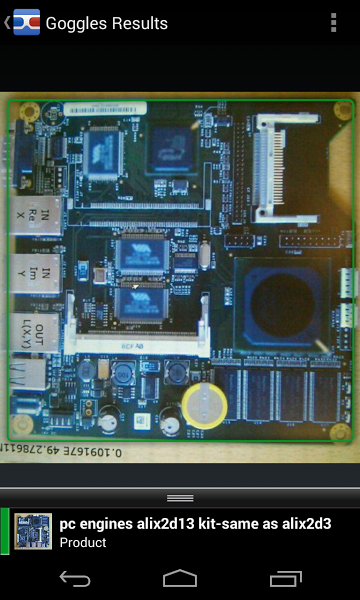
\includegraphics[width=0.8\columnwidth]{img/circuit-board.png}
    \caption{The identified circuit board}
    \label{fig:circuit-board}
\end{figure}

This leaves investigating yet another set of geographic coordinates: $0.109167E \; 49.278611N$. Learning from their previous experience, the geographic team decided to book a flight this time. They, of course, did not learn from their \emph{other} mistake, and hence spent quite some time travelling instead of taking the more sensible option of employing a parallel depth first search on the earth's map. The fact was reflected appropriately in their performance review. But we digress \ldots

\begin{figure}[h]
    \centering
    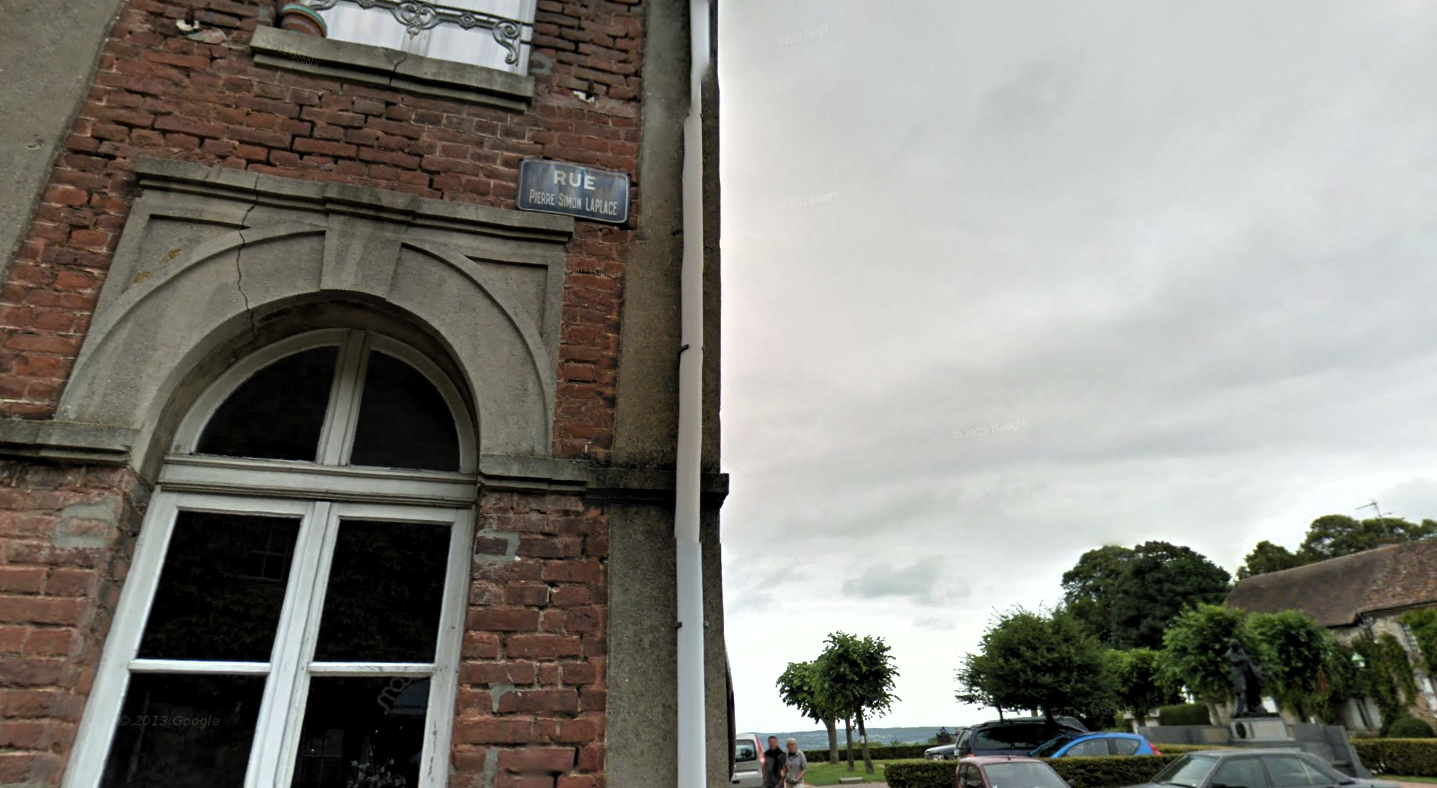
\includegraphics[width=0.95\columnwidth]{img/laplace-road.png}
    \caption{Rue Pierre Simon Laplace Road - You will never find a more blessed hive of charm and harmony}
    \label{fig:laplace-road}
\end{figure}


After an expensive trip to France, it was determined that the site referred to ``Ecole Beaumont en auge'' at ``Rue Pierre Simon Laplace Road'' (Figure~\ref{fig:laplace-road}). The connection was made the following week, when the team realised that the circuit was meant to employ some form of Laplace transform.


\subsection{Circuit board microanalysis}

With the macroanlysis out of the way, our experts studied the circuit board's functionality through means of the reconstructed \texttt{mystery.o} object file.



\subsubsection{\texttt{strings} analysis}
Executing \texttt{strings} analysis on \texttt{mystery.o} revealed the following hidden data:

\begin{quote}
\texttt{(C) 2006 Svenska Aeroplan AB (SAAB) Designad av Margarita Gonz\'{a}lez Sampayo, Linkoping}
\end{quote}

The English translation:
\begin{quote}
\texttt{(C) 2006 Swedish Aeroplane Company Limited (SAAB) Designed by Margarita Gonz\'{a}lez Sampayo, Linkoping}
\end{quote}


A background search revealed that Dr. Margarita Holmberg (Gonz\'{a}lez Sampayo was her maiden name) had centred her PhD thesis\footnote{Engineering problem solving
- The case of the Laplace transform as a difficulty in learning in electric circuits and as a tool to solve real world problems} around the Laplace Transform in electric circuits. Indeed, it seems that SAAB is mentioned twice in her thesis, in the context of a practical application of the Laplace transform:

\begin{quote}
To solve problems working in Companies applying automatic control (for example, working in SAAB with aircraft dynamics) you use the Laplace transform.
\end{quote}




\subsubsection{\texttt{objdump} analysis}
The symbol table of \texttt{mystery.o} was extracted using \texttt{objdump --syms}. This revealed a number of interesting library functions being used:
\begin{itemize}
\item Mathematical functions, often operating on complex numbers, such as \texttt{cexp}, \texttt{muldc3}, \texttt{log}, and others.
\item Time-related functions, \texttt{time}, \texttt{strftime}, \texttt{strtol}, and \texttt{localtime})
\end{itemize}

Whilst the mathematical functions were to be expected, the time-related functions came as a surprise to our agents. This discovery motivated further, more dynamic, investigation.


\subsubsection{\texttt{ltrace} analysis}
By running \texttt{ltrace} whilst running the team obtained the library calls used during the computation phase. The first and subsequent runs are almost identical, apart from an extra initialisation step. The initialisation step includes a call to \texttt{localtime}, protected by \texttt{cxa\_guard} calls, which are used ``to support thread-safe, one-time initialization of function scope variables''\footnote{\url{http://www.opensource.apple.com/source/libcppabi/libcppabi-14/src/cxa_guard.cxx}} (Figure~\ref{fig:l-calls}).


\begin{figure}[h]
    \centering

    \begin{tabular}{cc}
    \toprule
    Initial call & Subsequent calls \\

    \midrule

    \texttt
        time                                    & time        \\
        {\color{red} \_\_cxa\_guard\_acquire }  &             \\
        {\color{red} localtime }                &             \\
        {\color{red} \_\_cxa\_guard\_release }  &             \\
        strftime                                & strftime    \\
        strftime                                & strftime    \\
        strtol                                  & strtol      \\
        strtol                                  & strtol      \\
        \_\_muldc3                              & \_\_muldc3  \\
        cexp                                    & cexp        \\
        cexp                                    & cexp        \\
        \_\_divdc3                              & \_\_divdc3  \\
        \_\_muldc3                              & \_\_muldc3  \\
        \_\_muldc3                              & \_\_muldc3  \\
        sincos                                  & sincos      \\
        log                                     & log         \\
        cexp                                    & cexp        \\
        \_\_divdc3                              & \_\_divdc3  \\
        \_\_muldc3                              & \_\_muldc3  \\
        cexp                                    & cexp        \\
        \_\_muldc3                              & \_\_muldc3  \\
    \bottomrule
    \end{tabular}

    \caption{Trace of library calls for the initial and subsequent calls of the function \texttt{L()} . The extra library calls performed in the first function call are highlighted in red.}
    \label{fig:l-calls}
\end{figure}
